%\input{/Users/joshyv/Research/misc/latex_paper.tex}
\documentclass{article}
\usepackage{amsmath}
\usepackage{graphicx}
\usepackage{amsfonts}
\usepackage{amssymb}
\usepackage{amsthm}
%\usepackage{cite}
\usepackage{algorithm}
\usepackage{algorithmic}
\usepackage{times}
\usepackage{fancyhdr}
\usepackage{graphicx}
\usepackage{verbatim}
\usepackage{color}
\pagestyle{fancy}

\oddsidemargin=0.0in %%this makes the odd side margin go to the default of 1inch
\evensidemargin=0.0in
\textwidth=6.5in
\headwidth=6.5in
\textheight=9in %%sets the textwidth to 6.5, which leaves 1 for the remaining right margin with 8 1/2X11inch paper
\headheight=12pt
\topmargin=-0.25in
%\headheight=0in
%\headsep=0in
%\pagestyle{headings}

\usepackage{hyperref}
% \usepackage{ulem}
% \usepackage{color}

% \newcommand{\loo}{$L^{(1)}_{h; \mD_n}$}
\newcommand{\conv}{\rightarrow}
% \newcommand{\Real}{\mathbb{R}}
% \providecommand{\tr}[1]{\textcolor{red}{#1}}

\newcommand{\mB}{\mathcal{B}}
\newcommand{\mD}{\mathcal{D}}
\newcommand{\mM}{\mathcal{M}}
\newcommand{\PP}{\mathbb{P}}           % probability
\newcommand{\EE}{\mathbb{E}}           % expected value
\newcommand{\II}{\mathbb{I}}           % expected value
\newcommand{\Real}{\mathbb{R}}           % expected value

\newcommand{\del}{\delta}
\newcommand{\sig}{\sigma}
\newcommand{\lam}{\lambda}
\newcommand{\gam}{\gamma}
\newcommand{\eps}{\varepsilon}

\providecommand{\mc}[1]{\mathcal{#1}}
\providecommand{\mb}[1]{\boldsymbol{#1}}
\providecommand{\mbb}[1]{\mathbb{#1}}
\providecommand{\mv}[1]{\vec{#1}}
\providecommand{\mh}[1]{\widehat{#1}}
\providecommand{\mt}[1]{\widetilde{#1}}
\providecommand{\mhc}[1]{\hat{\mathcal{#1}}}
\providecommand{\mhb}[1]{\hat{\boldsymbol{#1}}}
\providecommand{\mvb}[1]{\vec{\boldsymbol{#1}}}
\providecommand{\mtb}[1]{\widetilde{\boldsymbol{#1}}}

\newcommand{\argmax}{\operatornamewithlimits{argmax}}
\newcommand{\argmin}{\operatornamewithlimits{argmin}}


% \newcommand{\mN}{\mathcal{N}}

\newcommand{\hL}{\widehat{L}}
\newcommand{\MeB}{\mM \overset{\varepsilon}{{\sim}}_{\PP} \mB}
\newcommand{\MsB}{\mM \overset{S}{\sim}_{\PP} \mB}
\newcommand{\MnoteB}{\mM \overset{\varepsilon}{{\not\sim}}_{\PP} \mB}
\providecommand{\tr}[1]{\textcolor{black}{#1}}
\providecommand{\norm}[1]{\left \lVert#1 \right  \rVert}
\newcommand{\T}{^{\ensuremath{\mathsf{T}}}}           % transpose

\newtheorem{defi}{Definition}
\newtheorem{thm}{Theorem}
\newtheorem{thex}{Thought experiment}
\lhead{Vogelstein JT, et al}
\rhead{Statistical Supervenience}

\title{Are mental properties supervenient on brain properties?}

\author{Joshua T. Vogelstein$^1$, R. Jacob Vogelstein$^2$, Carey E. Priebe$^1$\\
$^1$Department of Applied Mathematics \& Statistics, \\ Johns Hopkins University, Baltimore, MD, 21218,\\ $^2$National Security Technology Department, \\ Johns Hopkins University Applied Physics Laboratory, Laurel, MD 20723
}

\begin{document}

\maketitle
%\tableofcontents
\begin{abstract}

The ``mind-brain supervenience'' \tr{conjecture} suggests that all mental properties (e.g.\ consciousness, intelligence, personality, etc.) are derived from the physical properties of the brain. The validity of this \tr{conjecture} has been argued in philosophical terms for over 2,500 years. \tr{Alternative conjectures, including various non-physical causes of mental properties, seem rather implausible to many, but proving or disproving these alternatives has remained elusive.}  


To enable addressing the question of whether the mind supervenes on the brain through empirical means, here we frame a supervenience hypothesis in rigorous mathematical terms and propose a modified version of supervenience (called $\varepsilon$-supervenience) that is amenable to empirical investigations and statistical analysis. To elucidate this approach, we posit a thought experiment that illustrates how the probabilistic theory of pattern recognition can be used to make a one-sided determination of $\varepsilon$-supervenience. The physical property of the brain employed in this analysis is the graph describing brain connectivity (i.e., the brain-graph or \emph{connectome}), and $\varepsilon$-supervenience allows us to determine whether a particular mental property can be inferred from one's connectome to within any given misclassification rate $\varepsilon > 0$, regardless of the relationship between the two. %In addition to the theoretical results, we show via simulation that given reasonable assumptions about class conditional probabilities and the amount of data available, the thought experiment can actually be conducted on a simple organism, \emph{Caenorhabditis elegans}, with currently available technology.

The potential significance of this work can be divided into distinct disciplines.  To the philosopher, this work demonstrates an example of morphing philosophical conjectures into statistical hypotheses that are amenable to experimental investigations, allowing the philosopher to add empirical support to their rational arguments.  To the statistician, this work points out the limitations of hypothesis testing in a novel domain, and is suggestive of more general limitations previously (perhaps) under-appreciated.   To the neuroscientist, cognitive scientist and psychologist, this work indicates that much of contemporary research can be considered supervenience investigations, further motivating brain-graph related research paradigms.



\end{abstract}

% \vspace*{0.5 in}


\section{Introduction}

Questioning the relationship between the mind (our thoughts, beliefs, preferences, emotions, intelligences, etc.) and the brain (the physical structure inside our skulls) dates back at least as far as 400~BCE, when Plato wrote the dialogues, in which he posited immateriality of the soul \cite{Plato97}. Approximately two millennia passed before these ideas reached their canonical form through Descartes's discussion of mind-body dualism \cite{Descartes1641}. Then, in the 20th century, Donald Davidson stated and popularized the mind-brain supervenience \tr{conjecture}, which claims that an agent cannot alter in some mental property without altering in some physical property \cite{Davidson70}. Contemporary fields of neural network theory and neuroscientific inquiry often assume mind-brain supervenience, or an even stronger assumption about mind-brain causality, but no previously proposed notion of supervenience seems amenable to empirical investigation. This work is an attempt to bridge the gap between these philosophical conjectures and experimentally testable hypotheses. % Here we define new versions of supervenience that formulate the \tr{conjecture} in rigorous mathematical terms, and that can be experimentally tested \tr{as a hypothesis}.

The primary contributions of this work are as follows.  A notion of supervenience amenable to empirical investigation is formally introduced.  This renders the mind-brain dualism debate a hypothesis, rather than an assumption, both expanding the space of questions amenable to hypothesis testing, and placing limits on this space.  Because hypothesis tests (implicitly sometimes) depend on a model, a very general model of brains and their associated mental properties is proposed.  Fortunately, this formulation admits universally consistent classifiers, that is, classifiers guaranteed to find the relationship between minds and brains, if one exists, given sufficient data.  Many previous investigations relating brains and mental properties can therefore be considered $\eps$-supervenience hypothesis tests.  This paradigm, therefore, generalizes previous approaches, embedding them in a rigorous statistical framework, suggesting avenues for future research.


 % we demonstrate through simulation that the proposed universally consistent classifier has reasonable convergence properties on simulated brain-graph data. Finally, we discuss both contemporary and future applications of this framework to neurobiological studies in humans.


\section{Statistical supervenience} % (fold)
\label{sec:preliminaries}

% \subsection{Mind Brain Supervenience} % (fold)
% \label{sub:supervenience}

% subsection supervenience (end)
% The intention in this work is to develop greater insight regarding the relationship between minds and brains, using statistical methods, with particular interest in notions of supervenience.  Modern philosophy of science suggests that adequate scientific explanations must account for the objects of investigation and their relationships \cite{Craver07}. Therefore, here we define minds, brains, and supervenience.
% The mind-brain supervenience conjecture is a relation between the set of mental states and the set of brain states.  

Donald Davidson canonized the mind-brain supervenience relation in 1970 with the following quote: \cite{Davidson70}
\begin{quotation}
\noindent supervenience might be taken to mean that there cannot be two events alike in all physical respects but differing in some mental respect, or that an object cannot alter in some mental respect without altering in some physical respect.
\end{quotation}
This conjecture may be concisely and formally stated.  Let $b$ correspond to an agent's brain, which is a particular element from the set of all possible brains, $\mB$. % The set of possible brains $\mB$ is completely unrestricted, meaning that $\mB$ could be an infinite set, with arbitrarily complexity.  In particular, $b$ might represent the position, momentum, and type of each subatomic particle residing within the skull some agent.  %Thus, each different $b \in \mB$ could correspond to some difference in the position, momentum, or type of at least one subatomic particle composing the brain.
Similarly, let $m$ correspond to an agent's mind, which is a particular element from the set of all possible minds, $\mM$.  %The set of possible minds $\mM$ is also unrestricted. In particular, $m$ might represent all an agent's thoughts, beliefs, and preferences. %Thus, each different $m \in \mM$ could correspond to a difference in at least one thought, belief, or preference. 
Thus%, the above mind brain supervenience conjecture may be formally stated
: $m \neq m' \implies b \neq b' \, \forall (m,b) \neq (m',b') \in \mc{M} \times \mc{B}$, where $(m,b)$ and $(m',b')$ are mind-brain pairs.  This mind-brain supervenience relation does not imply an injective relation, a causal relation, or an identity relation (see Appendix \ref{sec:relations} for more details).

To facilitate both statistical analysis and empirical investigation, we convert this supervenience relation from a logical to a probabilistic relation.  Let $\PP[M,B]$ indicate a joint distribution of minds and brains.
%Each distribution $\PP[M,B]$ uniquely specifies the probability of any element $(m,b)$ occurring from the space of all possible elements $\mc{M} \times \mc{B}$. % (also called the \emph{sample space}).%  The true distribution could in theory be any possible joint distribution from the model, $\PP[M,B] \in \mc{P}$, meaning that we only assume that it conforms to the \emph{probability axioms}:
% \begin{enumerate}
% 	\item $0 \leq \PP[B=b,M=m] \leq 1$ for all $(m,b) \in \mM \times \mB$
% 	\item $\PP[\Omega]=1$ and $\PP[\emptyset]=0$, where $\Omega$ is the whole sample sample, that is, all elements, $(m,b) \in \mc{M} \times \mc{B}$
% 	\item any countable sequence of pairwise disjoint elements, $(m_1,b_1), (m_2,b_2), \ldots$ satisfies \\
% 	\mbox{$\PP[(m_1,b_1) \cup (m_2,b_2) \cup \ldots] = \sum_i \PP[(m_i,b_i)]$}.
% \end{enumerate}
%Given a distribution, one can then calculate any marginal or conditional distributions.  For instance, $\PP[B]=\int_{m \in \mM} \PP[M,B]dm$, or $\PP[M|B]=\PP[M,B]/\PP[B]$.  Having specified a model, statistical supervenience can be defined as follows:
\begin{defi}
\label{def1} 
$\mM$ is said to \textit{statistically supervene} on $\mB$ for distribution $\PP=\PP[M,B]$, denoted $\mM \overset{S}{\sim}_\PP \mB$, if and only if $\PP[m \neq m' | b=b']=0$, or equivalently $\PP[m = m' | b = b']=1$, for all $(m,b) \neq (m',b') \in \mc{M} \times \mc{B}$.
\end{defi}
\noindent Statistical supervenience is therefore a probabilistic relation on sets (related to, but distinct from correlation; see Appendix \ref{sec:relations} for details).  

 % Consider the following analogy: one desires to understand the relationship between height and weight.  In such a scenario, height, $h$, could be assumed to be an element from the set of all possible heights, $\mc{H}=(0,\infty)$ cm; and weight, $w$, could be assumed to be an element from the set of all possible weights, $\mc{W}=(0,\infty)$ kgs.   Then, it may be assumed that an agent's height and weight is sampled identically and independently from some \emph{model}, that is $(h,w)\overset{iid}{\sim}\PP[H,W]=F_{HW}$. To gain insight into $F_{HW}$, one might then state hypotheses, collect data, and perform analyses.  Implicit in the exposition of a model is that both objects, height and weight here, are \emph{random objects}.  Note that this does not imply anything in particular about the distribution (which could be a point mass, for instance); rather, it is a formal definition necessary for statistical analysis and empirical investigation. 
% 
% \subsection{Brain-graphs} % (fold)
% \label{sub:brain_graphs}


% subsection brain_graphs (end)

% section preliminaries (end)

%\section{Results}

\section{Statistical supervenience is equivalent to perfect classification accuracy} % (fold)
\label{sub:theoretical_results}

% subsection theoretical_results (end)
If minds statistically supervene on brains, $\MsB$, then two different minds must supervene on two different brains.  This means that there exists a unique mapping from each brain to a single mind.  In other words, one can in principle construct a function $g(b): \mB \mapsto \mM$, that is a deterministic mapping from brains to minds.  It may be the case that subsets of brains form equivalence classes, such that any brain in that subset is mapped to the same mind (see Appendix \ref{sec:relations} for examples).  Assuming for the moment that the space of all possible minds is finite, that is $| \mM| < \infty$, then we call any such function a \emph{classifier} (this assumption will later be relaxed).  Let $\mh{m}$ denote the output of a classifier, $g(b)=\mh{m}$.  Define misclassification rate as:
% \begin{align}
	$L_{\PP}(g) = \PP[g(B) \neq M]$, %= \frac{1}{|\mB| |\mM|}\iint \II\{g(b)\neq m\} db dm
% \end{align}
% where $\II\{\cdot\}$ indicates the indicator function, taking unity value if its argument is true, and zero otherwise.  
% $L_{\PP}(g)$ therefore effectively 
which counts the fraction of time $g$ misclassifies $b$. The Bayes optimal classifier $g^*$ minimizes $L_{\PP}(g)$ over all classifiers, that is:
% \begin{align}
	$g^* = \argmin_{g} L_{\PP}(g)$.
% \end{align}
% where $\mc{G}$ is the set of all possible classifiers.  
Thus, the \emph{Bayes error}, or Bayes risk, $L_{\PP}(g^*)$ is the minimum possible misclassification rate. The primary result of casting supervenience is a statistical framework is the following theorem: 
\begin{thm}
\label{thm1} 
$\mM$ is said to \textit{statistically supervene} on $\mB$ for distribution $\PP=\PP[M,B]$, denoted $\mM \overset{S}{\sim}_{\PP} \mB$, if and only if $L_{\PP}(g^*) = 0$. Formally, \mbox{$\MsB \Leftrightarrow L_{\PP}(g^*)=0$}.  
\end{thm}
% \begin{thm} 
% 	\label{thm1} 
% 	Statistical supervenience implies that there exists a classifier that is \emph{always correct}, that is, $g(b)=m$, for all $(m,b) \in \mc{M} \times \mc{B}$.  
% \end{thm}

\noindent If minds supervene on brains, then, by the definition of supervenience, there exists a function that maps each brain deterministically to a particular mind.  This means that one could draw a decision boundary between all equivalence classes of brains, each class corresponding to a different mind, and no mind will reside within two different equivalence classes.  Thus, the optimal classifier would correctly find these decision boundaries, and therefore have no opportunity to err. $\square$

Thus, the above arguments shows (for the first time to our knowledge) that statistical supervenience and zero Bayes error are equivalent. Further, statistical supervenience can be thought of as a constraint on the possible models.  Specifically, let $\mc{P}$ indicate the set of all possible joint distributions on minds and brains, and let $\mc{P}_s$ be subset of models for which supervenience holds.  Then, $\mc{P}_s = \{\PP[M,B] : L_{\PP}(g^*)=0\} \subseteq \mc{P}$.


\section{A hypothesis test for supervenience} % (fold)
\label{sub:hypothesis_testing}

While the above theorem is of potential theoretical interest, because the arguments rest on knowing $\PP[M,B]$ and $g^*$, which are typically unknown, they are pragmatically useless.  However, both $\PP[M,B]$ and $g^*$ could be estimated from data.  Let $\mc{T}_n=\{(m_1,b_1), (m_2,b_2), \ldots, (m_n,b_n)\}$ be a set of random samples taking their values in $\mc{M} \times \mc{B}$, each independently and identically distributed according to model $\PP[M,B]$.  Generalizing the concept of a classifier $g$ to allow incorporation of training data, consider $g_n:\mB \times (\mc{M} \times \mc{B})^n \mapsto \mM$ which takes as input an observed brain  $b$ and training data $\mc{T}_n$, and produces a classification $g_n(b;\tr{\mc{T}_n})=\mh{m}$.  Misclassification rate for this classifier will be a random variable, because the training data $\mc{T}_n$ are random samples.  The expected misclassification rate for this classifier is therefore approximated by ``hold-out'' error:
% Therefore, instead of calculating misclassification rate for $g_n$, we compute the expected misclassification rate: % as the expectation of $\PP[g_n(B)=M | \mc{T}_n]$ over all possible training data corpuses:
% \begin{align}
% \EE[L_{\PP}(g_n)] = \EE[\PP_F[g_n(B;\tr{\mc{T}_n}) \neq M|\tr{\mc{T}_n}]] = \int \PP[g_n(B)=M | \mc{T}_n] \PP[\mc{T}_n] d\mc{T}_n.
% \end{align}
% Unfortunately, in practice, computing $\EE[L_{\PP}(g_n)]$, requires integrating over all possible training data corpuses of size $n$, and by definition, we only have access to a single training data corpus.  We therefore define ``hold out'' misclassification performance:
% \begin{align}
% \EE[L_{\PP}(g_n)] 
% &\approx  \hL^{n'}_{F}(g_n) = \sum_{\mc{T}_{n-n'}} \PP[g_n(B)=M | \mc{T}_{n-n'}] \PP[\mc{T}_{n-n'}],
% \end{align}
$\hL^{n'}_{F}(g_n) = \PP[g_n(B)=M | \mc{T}_{n-n'}]$,
where $n'<n$ is the number of held-out training samples (samples not used to obtain $g_n(\cdot)$).
%, and the sum is taken over a sufficiently large number of subsets, $\mc{T}_{n-n'}$, such that $\hL^{n'}_F(g_n)$ converges.  
 % $n' \hL^{n'}_{F}(g_n)$ is t
The approximate expected number of misclassified minds
%. Simplifying further by assuming just one hold-out set, then $n' \hL^{n'}_{F}(g_n)$ 
therefore
% and 
has a binomial distribution:  $n' \hL^{n'}_{F}(g_n) \sim \text{Binomial}(n',L_{\PP}(g_n))$. %, because for any of the $n'$ held-out samples, the classifier could be either correct or incorrect.

Before explicitly considering the problem of testing for statistical supervenience, we define a relaxed notion of supervenience:
\begin{defi}
\label{def2}
Given $\varepsilon > 0$, $\mM$ is said to $\varepsilon$-\textit{supervene} on $\mB$ for distribution $\PP=\PP[M,B]$, denoted $\MeB$, if and only if $L_{\PP}(g^*) < \varepsilon$.
\end{defi}

Given this relaxation, consider the problem of testing for $\eps-$supervenience.  %First, specify a significance level, $\alpha$, such that if the p-value is less than $\alpha$, then the null is rejected.  
% Because we hope to reject the null, in favor of the alternative, l
Let the null hypothesis be $H_0$: $L_{\PP}(g_n) \geq \eps$, and the alternative hypothesis be $H_A$: $L_{\PP}(g_n) < \eps$.  We reject for  values of the test-statistic lower than the critical value, that is, we reject if and only if $n' \hL^{n'}_{F}(g_n) <c_{\alpha}(n',\varepsilon)$.  The critical value is available under the least favorable distribution $\text{Binomial}(n',\varepsilon)$.  Thus, rejection implies that we are $100(1-\alpha$)\% confident that $\MeB$.  The definition of $\eps$-supervenience therefore admits, for the first time to our knowledge, a statistical test of supervenience, given a specified $\eps$ and $\alpha$. %Similar to the above, one can define the set of $\eps$-supervenience models as the set of models under which $\eps$-supervenience holds, that is: $\mc{P}_\eps = \{\PP | L_{\PP}(g^*)< \eps\}$.  One could then sort  $\eps$-supervenience subsets,  $\mc{P}_s \subseteq \mc{P}_{\eps} \subseteq \mc{P}_{\eps'} \subseteq \mc{P}$, for any $\eps < \eps'$.

% subsection hypothesis_testing (end)

% \section{Power and consistency} % (fold)
% \label{ssub:power_and_consistency}

	
	
Importantly, the utility of any statistical test depends both on the p-value, the probability of obtaining a test statistic at least as extreme as the observed value (under the assumed model), and its power, the probability that the test will reject a false null hypothesis% (in other words, the probability that it will not make a Type II error)
.  Ideally, the power of this test would go to unity, as $n,n' \rightarrow \infty$.  A sufficient condition for power to approach unity is that $g_n$ is a \emph{consistent} classifier.  A classifier is consistent if and only if its expected misclassification rate converges to the Bayes optimal limit with sufficient data, that is $\EE[L_{\PP}(g_n)] \conv L_{\PP}(g^*)$ as $n\conv \infty$. %As the notation suggests, consistency of a classifier is a function of the true model, $\PP$.  Without any prior knowledge of what the model might be, one desires a \emph{universally consistent} classifier, that is a classifier that is consistent for all $\PP \in \mc{P}$.  
% The above described hypothesis tests suggests the following theorem:
% 
% \begin{thm} \label{thm1} 
% Given $\alpha > 0$, we can test $\MeB$ so that rejection implies $\MeB$ holds with probability greater than or equal to $1-\alpha$. Furthermore, given a consistent classifier the power of the test converges to unity. 
% \end{thm}


Unfortunately, the rate of convergence of $L_{\PP}(g_n)$ to $L_{\PP}(g^*)$ depends on the (unknown) distribution $\PP=\PP[M,B]$ \cite{DGL96}. Furthermore, arbitrarily slow convergence theorems regarding the rate of convergence of $L_{\PP}(g_n)$ to $L_{\PP}(g^*)$ demonstrate that there is no universal $n,n'$ which will guarantee that the test has power greater than any specified target $\beta > \alpha$ \cite{Devroye83}. For this reason, the test outlined above can provide only a one-sided conclusion: if we reject we can be $100(1-\alpha)$\% confident that $\MeB$ holds, but we can never be confident in its negation; rather, %.  This means that we can never be confident that $\MeB$ does \emph{not} hold; rather, 
it may be the case that the evidence in favor of $\MeB$ is insufficient for any number of reasons, including that we simply have not yet collected enough data. %Unfortunately, arbitrarily slow convergence theorems inform us that no matter how much data we collect, we cannot disambiguate between not yet having enough data, and $\MeB$ not holding.  
Thus, without restrictions on $\PP[M,B]$, arbitrarily slow convergence theorems imply that our theorem of $\varepsilon$-supervenience does not \tr{strictly} satisfy Popper's {\it falsifiability} requirement \cite{Popper}. %Given these limitations on even universal consistency, it is still the best one can hope for.  Therefore, we hope to obtain a universally consistent classifier to test for $\eps$-supervenience.

% subsubsection power_and_consistency (end)


\section{A thought experiment to guarantee unity power} % (fold)
\label{sub:uc}

% Below, we will assume that brains are characterized by graphs, referred to hereafter as ``brain-graphs.''  This assumption follows naturally from the neuron-doctrine
% % Given the above notion of statistical supervenience, one can then design a statistical test for supervenience by carefully considering an appropriate model.  For mind-brain supervenience, a model of the brain is paramount, and has historically been a bit of a sticky wicket.  It was not until 1891, that H.~Waldeyer-Hartz first formally proposed the ``neuron doctrine'' 
% \cite{Waldeyer-Hartz1891}, which states that the nervous system is a complex {network} of neurons, largely based on Ramon y Cajal's work using the Golgi stain \cite{Finger01}.  This doctrine has been central to much of the development of neuroscience and artificial intelligence for over 100 years, including the development of neural network theory \cite{Bishop95} and cognitive science \cite{McClellandRumelhart86}.  %Fundamental to nearly all models of the brain (or components therein) since the neuron doctrine's introduction is the existence of neural units, each connected to (some) other neural units.  Therefore, it seems appropriate to assume that a reasonable model of a brain is graph, composed of a set of vertices (or nodes), each representing a neural unit, and a set of edges (arcs) connecting the nodes.  Below, we formalize this concept to enable statistical testing in the graph domain.
% Below, we will assume that $m$ is binary, that is, $m \in \{0,1\}$ (for example, $m$ might indicate whether the person knows calculus or not).

To ensure consistency and therefore unity power, the classifier $g_n(\cdot)$ must be able to converge to the truth, regardless of the true model, $\PP$.  We therefore make explicit a model for brain, and show that under this very general model, universally consistent classifiers are available.

\begin{thex}
Let the physical property under consideration be brain connectivity structure (``connectome''), so $b$ is a brain-graph \tr{(or, network)} with vertices representing neurons (or neuroanatomical regions) and edges representing synapses (or white matter tracts). Further let $\mB$, the observation space, be the collection of all graphs on a finite number of vertices, and let $|\mB|$ be countable. Now, imagine collecting very large amounts of very accurate independent and identically distributed brain-graph data and the associated mental property indicators. A $k_n$-nearest neighbor classifier using an isomorphism-matching Frobenius norm is universally consistent (see Appendix \ref{sec:knn} for proof). Therefore, %Theorem \ref{thm1} applies and 
the existence of a universally consistent classifier guarantees that eventually (in $n,n'$) we will be able to conclude $\MeB$ for this mental/brain property pair, if indeed $\varepsilon$-supervenience holds. This logic holds for directed graphs or multigraphs or hypergraphs with discrete edge weights and vertex attributes. Furthermore, Appendix \ref{sec:knn} also extends the proof to deal with other matrix norms (which might speed up convergence), and the regression scenario, where $|\mM|$ is infinite.  
\end{thex}

%(fold)
% Formally, a brain-graph $G=(V,A)$ is characterized by a set of vertices (or nodes), $V = \{V_i\} = \{V_1,\ldots, V_n\}$, where $n$ is the number of neural units, and arcs (or edges) $A=\{A_{ij}\}$, where $A_{ij}$ represents the connectivity from neural unit $V_j$ to $V_i$. For simplicity (to be generalized below), assume that brain-graphs are simple graphs, meaning that for all $i,j \in [n]$: (i) there are no self loops, $a_{ii}=0$, (ii) all edges are binary, $a_{ij} \in \{0,1\}$, and (iii) all edges are symmetric,  $a_{ij}=a_{ji}$.  Further assume that the vertices are \emph{labeled}, meaning that there is a known one-to-one mapping from each vertex in any brain to a vertex in any other brain, and that each brain-graph has the same number of vertices.  Thus, each brain-graph is characterized entirely by its adjacency matrix, $a \in \mc{A}$, where $\mc{A} \subseteq \{0,1\}^{n \times n}$. Further, let the mental property under investigation be binary, so $m \in \mc{M} = \{0,1\}$.  The Bayes classifier is:
% \begin{align}
% 	\mh{m} = \argmax_m \PP[b,m] = \argmax_m \PP[b|m] \PP[m] 
% \end{align}
% where the likelihood term, $\PP[B|M]$, specifies the probability of observing any particular adjacency matrix for any class, and the prior term, $\PP[M]$, specifies the prior probability of either class.  
% 
% Under the above model assumptions, the number of possible brain-graph/mental-property pairs is finite, that is, $|\mc{M} \times \mc{B}| = d < \infty$.  Therefore, one can simply enumerate all possible brain-graphs for each class, such that each class is represented by a multinomial distribution.  The maximum likelihood estimator (MLE) of the multinomial parameter for each class as guaranteed to converge to the true (but unknown) parameter.  Formally, one can state $\mh{\PP}_{MLE}[B|M] \conv \PP[B|M]$ as $n \conv \infty$, almost surely.  Furthermore, the MLE  estimator of the prior also converges to the true (but unknown) prior distribution, $\mh{\PP}_{MLE}[M] \conv \PP[M]$, as $n \conv \infty$, almost surely.  
% 
% The Bayes plugin classifier is defined by:
% \begin{align}
% 	\mh{m} = \argmax_m  \mh{\PP}[b|m] \mh{\PP}[m] 
% \end{align}
% where $\mh{\PP}[B|M]$ and $\mh{\PP}[M]$ are plugin estimators.  Since the MLE estimators defined above are plugin estimators, and consistent, one obtains a consistent classifier by plugging in the MLE parameters.  This logic holds for any model in which the cardinality of the sample space is finite, that is $|\mc{M}\times \mc{B}| < \infty$.  In particular, one can relax both the assumed symmetry and hollowness of the adjacency matrix, and this result still holds.  Furthermore, one can allow for multi-graphs, in which there are a finite number of different kinds of edges (different colored edges), such that $a_{ij} \in \{0,1,\ldots, K\}$, with $K < \infty$, and the set of possible brain-graphs remains finite.  Finally, one can allow $\mc{M}$ to be any finite space, not just binary.  Note that in all these cases, the process one uses to enumerate and sort the brain-graph collections is essentially irrelevant, assuming the same process is used for each class.  Further note that more robust estimators, such as certain M-estimators and the \emph{maximum a posteriori} estimators, also admit universally consistent classifiers, with perhaps faster convergence properties.
% 
% The above approach, however, is insufficient in several important cases.  First, when the edges live in a continuous space, such as $a_{ij} \in \Real$, corresponding to weighted graphs, the MLE plugin is not well defined.  In such scenarios, the $k_n$ nearest neighbor ($k$-NN) algorithm can be used (see Appendix 1 for a description of the $k$-NN algorithm) \cite{Stone77}.  Although originally defined to operate on finite dimensional Euclidean space, the same algorithm can be applied here, once one has first embedded the brain-graphs into such a space.  One possible embedding is to stack the columns of the adjacency matrix, yielding an $n^2$ element vector, instead of an $n \times n$ element matrix.  Given such an embedding, the $k$-NN classifier may be used without modification, assuming one has defined a suitable distance operator (such as $L_2$ or $L_1$).  This algorithm may also be used in the above cases where the support of the sample space is finite, and, convergence of the $k$-NN algorithm for those problems will be faster than the MLE plugins, whenever the distance used is ``appropriate'' (where appropriate is assessed by convergence rates under the true (but unknown) model).  Furthermore, one can allow for multiple kinds of edges, as before, yielding adjacency tensors, with $a_{ij} \in \Real^d$.  Or, one can allow the mental property to be multidimensional as well, $m \in \Real^l$.  The $k$-NN algorithm converges in both these generalizations.  Finally, one could allow the number of vertices to differ across brain samples.  In such a scenario, one can ``pad'' the adjacency matrices of the smaller brain-graphs, and the result still holds.  
% 
% The above universal consistency results hold for unlabeled graphs as well, with a minor modification. Assuming the brain-graphs are unlabeled, and we have a test brain-graph $b$, one could first align each training brain-graph with the test brain-graph, and then use the above algorithms.  To align any pair of graphs, one can solve the graph isomorphism problem, $\mh{Q}_i=\argmin_{Q \in \mc{Q}} \norm{Q b_i Q\T - b}$, where $\mc{Q}$ is the set of all permutation matrices (that is, zero matrices with a single unit value in each row and column).  Given $\mh{Q}_i$, one can compute $\mt{b}_i=\mh{Q}_i b \mh{Q}_i\T$, and then proceed as one would normally.  Unfortunately, the graph isomorphism problem is known to be NP-incomplete (that is, it is not known to believe in either P or NP-complete) \cite{GareyJohnson79}, and therefore no polynomial time algorithm is available, making this approach quite time-consuming.
% 
% 
% % subsection brain_graphs 
% 
% \section{Theoretical implications} % (fold)
% \label{sub:implications}
% 
% Returning to the question of supervenience, consider the following thought experiment.  Let the physical property under consideration be brain-graphs, and the mental property under investigation be binary (such as, knows calculus or not). Now, imagine collecting very large amounts of very accurate exchangeable brain-graph data and the associated mental property values. A $k_n$-nearest neighbor algorithm using an isomorphism-matching Frobenius norm is universally consistent. Therefore, %Theorem \ref{thm1} applies and 
% the existence of a universally consistent classifier guarantees that eventually (in $n,n'$) one will be able to conclude $\MeB$ for this mental/brain property pair, if indeed $\varepsilon$-supervenience holds. This logic holds for directed graphs or multigraphs or hypergraphs with edge weights, with or without labeled vertices. 
% 
% 
% % subsection implications (end)
% 
% 
% % subsection practical_applications (end)
%(end)

\section{Discussion}

\subsection{Summary} % (fold)
\label{par:summary}

We have introduced the notion of $\eps$-supervenience, which states that the misclassification rate for any mental/brain property pair is less than $\eps$.  Furthermore, we have shown that $k$-NN classifiers are universally consistent, such that one can derive a hypothesis test, with confidence level $\alpha$, that is guaranteed to converge to the Bayes optimal misclassification rate, given sufficient data, no matter the true (but unknown) distribution of mental/brain pair properties.  Furthermore, this is a one-sided test, so although power converges to unity, one can never determine whether more data is necessary to get a lower $p$-value, or the particular $\eps$-supervenience does not hold.  

\subsection{Practical issues} % (fold)
\label{par:practical_issues}

Importantly, we are \emph{not} claiming that actually determining $\eps$-supervenience in humans when the vertices represent individual neurons is practically possible for any particular mental property at this time.  Rather, the claim is that \emph{if} one had sufficient data (a very large number of exchangeable mind/brain property pairs), then \emph{in theory}, some level $\eps$-supervenience hypothesis test could be performed.  Even in such a scenario, a universally consistent classifier is just one of many possible kinds of classifiers, and not necessarily the best one (in terms of $\mh{L}$), for any particular dataset.  Further, even if a universally consistent classifier is used, a more informative and tractable distance on $\mB$ may be desired, as the $k_n$-nearest neighbor classifier under an $L_p$ norm may have a rate of convergence so slow and a computational demand so high as to be impractical (though, see Appendix \ref{sec:sim} for a simulated example in which convergence is relatively fast).  Whichever classifier is used, it is likely to benefit from a large amount of domain specific knowledge, which the proposed classifier completely neglects.


% paragraph practical_issues (end)


% paragraph summary (end)

\subsection{A unified quest} % (fold)
\label{sub:practical_applications}

A central (perhaps \emph{the} central) quest in much of neuroscience, psychology, and cognitive science is to discover the brain properties that subvene under various mental properties, although questions are rarely cast in the supervenience formalism.  Moreover, the particular brain properties that are often believed to subvene under these mental properties are neural circuits, or brain-subgraphs.  To this end, many investigations in these fields include schematic diagrams showing a particular brain-subgraph subvening under a particular mental phenotype. This practice transcends the evolutionary hierarchy of neuroscientific research.  For instance, in the invertebrate literature, vertices correspond to particular labeled neurons, and edges correspond to synapse \cite{NorthGreenspan07}.  In the vertebrate literature, vertices tend to correspond to types of neurons in particular regions, and edges correspond to tendencies of connections \cite{Shepherd04}.  For primates \cite{Felleman_VanEssen91} and humans \cite{Mori05} vertices tend to represent functionally distinct neuroanatomical regions, and edges represent regional interconnectivity. Furthermore, this practice also transcends analytical background, including anatomists \cite{Abeles91}, philosophers \cite{Koch_Davis94}, statisticians \cite{Rao_Lewicki02}, and physicists \cite{Chow_Dalibard03}.  The near ubiquity of this practice suggests that a fundamental quest is to determine which brain-subgraphs subvene under which mental properties (perhaps causality, not supervenience, is the true desideratum).  



% \subsection{Causality} % (fold)
% \label{par:causality}
% 
% While the above thought experiment addresses the question of $\varepsilon$-supervenience, it does not address causality. Assuming we have confirmed $\MeB$ for a particular mental/brain property pair with confidence level $\alpha$, then morphing the brain (by altering edges) could be used to determine whether the relation is in fact causal.
% 
% % paragraph causality (end)

\subsection{Human applications} % (fold)
\label{par:human_applications}

In recent years, with the advent of the field of ``connectomics'' \cite{SpornsKotter05,Hagmann05}, neuroimaging has seen an explosion of studies investigating the human connectome, and relating connectomes to cognitive properties \cite{Jones10}.  These studies can all be thought of as testing various $\eps$-supervenience hypotheses.  For instance, a recent study showed that using data from diffusion tensor imaging \cite{Basser94}, one can nearly perfectly differentiate between schizophrenics and controls \cite{ArdekaniSzeszko10}.  As the resolution and signal-to-noise ratio of magnetic resonance imaging continues to improve, especially with more advanced techniques such as High Angular Diffusion Imaging \cite{TuchWedeen02}, Q-Ball Imaging \cite{Tuch04}, and diffusion spectrum imaging \cite{WedeenWeisskoff05}, similar results could be obtained with other, more subtle cognitive properties.  Furthermore, the utilization of other imaging technologies, such as polarized light imaging \cite{PalmAmunts10} and high-throughput electron microscopy \cite{DenkHorstmann04,HayworthLichtman06}, will continue to improve the effective resolution of these inferred connectomes from human brains. While determining whether a particular individual knows calculus might be quite distant, many other cognitive and psychological supervenience hypothesis have already been tested, and the gap between testing for calculus and testing for schizophrenia seems to be vanishing.




% paragraph relationship_to_previous_work (end)

\subsection{Quantum networks} % (fold)
\label{par:quantum_networks}

Recently, several authors have suggested the possibility that brains are better characterized as quantum networks, instead of classical networks \cite{Penrose,check_book}.  The above results hold regardless of whether computations in the brain are quantum or classical, as quantum networks merely speed up computation for certain classes of problems, they cannot, however, solve problems that classical computers cannot \cite{NielsenChuang00}.  This means, if the above analysis failed to reject the null at level $\alpha$, the interpretation does not change if one assumes quantum versus classical computations.



% paragraph quantum_networks (end)


\subsection{Stochastic Supervenience} % (fold)
\label{par:stochastic_supervenience}


Possible explanations of how it might be the case that $\eps>0$ include stochastic supervenience \cite{Craver09}, and supernatural causal effects.  Thus, the above analysis could be considered an empirical test for whether we have souls, or, perhaps whether souls play a causal role in our mental properties over and above the physical role played by the brain, or whether the data we have suggests that the probability that our souls play a measurable causal role over and above the physical is less than $\eps$.

% paragraph stochastic_supervenience (end)


\subsection{Dynamics vs. statics} % (fold)
\label{par:dynamics_vs_statics}

The above \emph{gedanken} experiment did not require simulating any dynamics; rather, the dynamics are necessarily a function of the model parameters (statics).  Similarly, for the question of mind-brain supervenience in humans, one need not ever observe any activity of the brain, one must merely observe the model, which determines the activity (in a potentially stochastic process). Thus, this approach to understanding the relationship between mind and brain is distinct from the standard systems neuroscience paradigm, in which the goal is typically to understanding the neural activity ``code.''  In contrast, if mind-brain supervenience is true, this motivates a search for the neural connectivity ``code,'' an \emph{engram} for memories \cite{Semon21, Lashley50, ZhangLinden03, ShemaDudai07, BerryDavis08}, or more generally a \emph{mengram}, the neural signature of any mental property, be it cognitive, psychological, or otherwise.  

% paragraph dynamics_vs_statics (end)

\subsection{Concluding thoughts} % (fold)
\label{par:concluding_thoughts}

% paragraph concluding_thoughts (end)

This thought experiment, together with (i) the formal definition of $\varepsilon$-supervenience, (ii) the brain-graph model, and (iii) the universal consistency proof on graphs, is the first demonstration (to our knowledge) that empirically investigating supervenience is at least theoretically possible. The above discussion suggests that many previously conducted investigations either assume supervenience, or test it.  Further, new technologies facilitate testing supervenience of mental properties on brain-graphs more easily.


\clearpage
\appendix



\section{Relations between sets} % (fold)
\label{sec:relations}

In this appendix we describe several kinds of relations that are not implied by supervenience.  

%For instance, it may be the case that minds supervene on brains, but one cannot form an \emph{injective} relation from brains to minds.  

First, a supervenient relation does not imply an injective relation.  An injective relation is any relation that preserves distinctness.  Thus if minds are injective on brains, then $b\neq b' \implies m \neq m' \, \forall (m,b), (m',b') \in \mc{M} \times \mc{B}$ (note that the directionality of the implication has been switched relative to supervenience). For instance, it might be the case that a brain could change without the mind changing.  Consider the case that a single subatomic particle shifts its position by a Plank length, changing brain state from $b$ to $b'$.  It is possible that the mental state supervening on brain state $b$ remains $m$, even after $b$ changes to $b'$.  In such a scenario, the mind might still supervene on the brain, but the relation from brains to minds is not injective. This argument also shows that supervenience is not necessarily a \emph{symmetric} relation.  Minds supervening on brains does not imply that brains supervene on minds.  


Second,  supervenience does not imply causality. %it may be the case that minds supervene on brains, but that brains do not cause minds.  
For instance, consider an analogy where $M$ and $B$ correspond to two coins being flipped, each possibly landing on heads or tails.  Further assume that every time one lands on heads so does the other, and every time one lands on tails, so do the other. This implies that $M$ supervenes on $B$, but assumes nothing about whether $M$ causes $B$, or $B$ causes $M$, or some exogenous force causes both.  

Third, supervenience does not imply identity.  Consider, for example, acceleration and velocity.  Clearly, acceleration supervenes on velocity, as acceleration cannot change without velocity changing (assuming one does not consider gravity as acceleration).  Similarly, velocity supervenes on position, as velocity cannot change without position changing.  Therefore, acceleration supervenes on position, by the transitive property of supervenience, but it is not the case that a change in acceleration is equal to a change in position.  Rather, position can change with constant velocity, meaning without acceleration changing.  

What supervenience does imply, however, is the following.   Imagine finding two different minds.  If $\MeB$, then the brains subvening under those two minds must be different.  In other words, there cannot be two different minds, either of which could supervene on a single brain.  Figure \ref{fig:rel} shows several possible relations between the sets of minds and brains.

\begin{figure}[htbp]
	\centering
		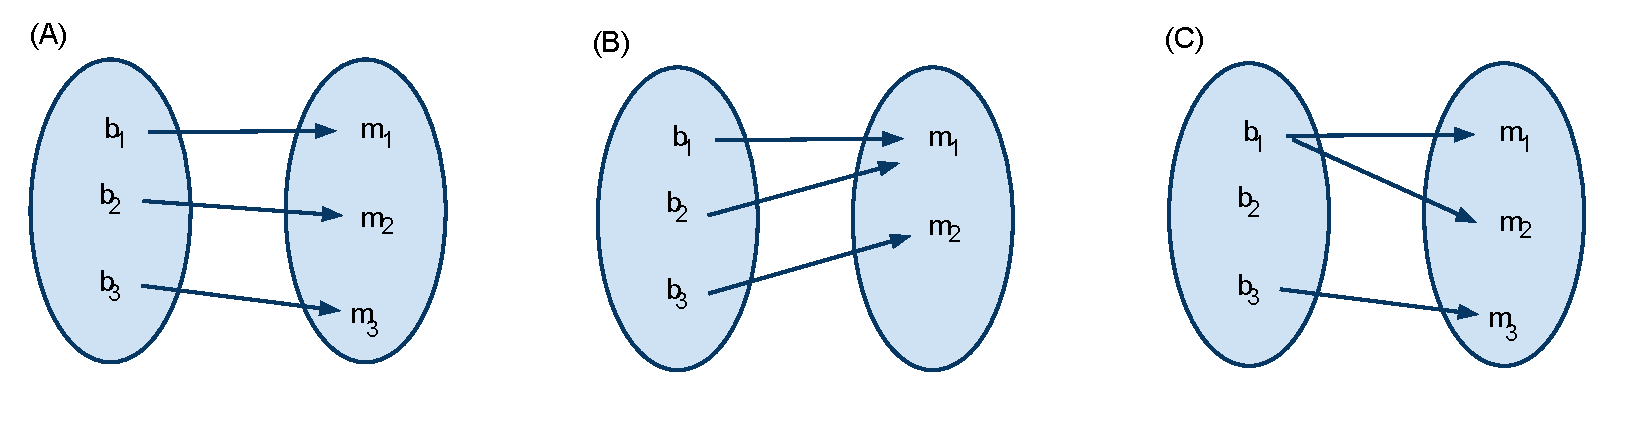
\includegraphics[width=1\linewidth]{supervenience_relations.pdf}
	\caption{Possible relations between minds and brains.  (A) Minds supervene on brains, and it so happens that there is a bijective relation from brains to minds.  (B) Minds supervene on brains, and it so happens that there is a surjective (a.k.a., onto) relation from brains to minds. (C) Minds are \emph{not} supervenient on brains, because two different minds supervene on the same brain.}
	\label{fig:rel}
\end{figure}
% section relations_between_sets (end)

Note that statistical supervenience is distinct from statistical correlation.  \emph{Statistical correlation} between brain states and mental states is defined as $\rho_{MB}=\EE[(B-\mu_B)(M-\mu_M)]/(\sig_B \sig_M)$, where $\mu_X$ and $\sig_X$ are the mean and variance of $X$, and $\EE[X]$ is the expected value of $X$.  If $\rho_{MB}=1$, then both $\MeB$ and $\mB \overset{\varepsilon}{{\sim}}_F \mM$. Thus, perfect correlation implies supervenience, but supervenience does not imply correlation.  


\section{$k_n$ nearest neighbor algorithm} % (fold)
\label{sec:knn}


% Assume that $b$ is a real $d$-dimensional vector, $b \in \mc{B} \subseteq \Real^d$, and $m$ is a binary indicator, $m \in \mc{M} = \{0,1\}$.  Then, further assume that we have observed a collection of training data, $\mc{T}_n =\{(m_i,b_i)\}_{i=1}^n$, each sampled identically and independently from some unknown joint distribution, $(m_i,b_i)\overset{iid}{\sim} \PP[M,B]$.  A new brain, $b$, called the ``test brain'', is then observed, and one desires to find the most likely class of the new brain, $m$.  It is further assumed that the test mind/brain pair is sampled from the same distribution as the training data, $(m,b)\sim \PP[M,B]$, and $m$ is simply unobserved.

The $1$-nearest neighbor ($1$-NN) classifier works as follows.  Compute the distance between the test brain and all the training brains, $d_i=d(b,b_i)$ for all $i \in [n]$, where $[n]=1,2,\ldots, n$.  Then, sort them, $d_{(1)} < d_{(2)} < \ldots < d_{(n)}$, and their corresponding mental properties, , $m_{(1)}, m_{(2)}, \ldots, m_{(n)}$, where parenthetical indices indicate rank order.  %One can then also obtain a rank order for the training minds, $m_{(1)}, m_{(2)}, \ldots, m_{(n)}$, where $m_{(i)}$ is the class of the $i^{th}$ closest training brain to $b$.  
The $1$-NN algorithm predicts that the unobserved mind is of the same class as the closest brain's class: $m=m_{(1)}$.  The $k_n$ nearest neighbor is a straightforward generalization of this approach.  It says that the test mind is in the same class as which ever class is the majority class of the $k_n$ nearest neighbors, $m=\II\{\sum_{i=1}^{k_n} m_{(i)} > k_n/2\}$.  Given a particular choice of $k_n$ (the number of nearest neighbors to consider), and a choice of $d(\cdot,\cdot)$ (the distance metric used to compare the test datum and training data), one then has a relatively simple and intuitive algorithm.  

Unfortunately, no such algorithm is universally consistent.  Let $g_n$ be the $k_n$ nearest neighbor classifier when there are $n$ training points.  Then, a collection of such algorithms, $\{g_n\}$,  with $k_n$ increasing with $n$, can be universally consistent under certain constraints. In particular, as $n$ increases, $k_n$ must also increase, but not quite as quickly.  Formally, $k_n$ must satisfy: (i) $k_n \conv \infty$ as $n \conv \infty$ and (ii) $k_n/n \conv 0$ as $n\conv\infty$. In Stone' original proof, the $L_2$ norm ($d(b,b')=\sum_{j=1}^d (b_j-b_j')^2$, where $j$ indexes elements of the $d$-dimensional vector) was shown to satisfy the constraints on a distance metric for this collection of classifiers to be universally consistent.  Later, others extended these results to apply to any $L_p$ norm \cite{DGL96}.  When brain-graphs are represented by their adjacency matrices, one can stack the columns of the adjacency matrices, effectively embedding graphs into finite Euclidean space, in which case Stone's theorem applies.
% section _k_n_nearest_neighbor_algorithm (end)

\section{Simulation} % (fold)
\label{sec:sim}

As an example of a feasible experiment, one may consider a species whose nervous system consists of the same (small) number of labeled neurons for each organism. {\it Caenorhabditis elegans} is believed to be such a species \cite{Durbin87}. The hermaphroditic C.~elegans' somatic nervous system consists of 279 interconnected neurons. While the graph with these neurons as vertices and edges defined by chemical synapses between neurons is not identical across individuals, it is reasonably consistent \cite{Durbin87}. Furthermore, these animals exhibit a rich behavioral repertoire that depends on circuit properties \cite{deBonoMaricq05}. Thus, one may design an experiment by describing the joint distribution $\PP[M,B]$ via class-conditional distributions $\PP[B|M=m_j]$ for the C.~elegans brain-graph for two mental properties of interest, $m_0$ and $m_1$, along with the prior probability of class membership $\PP[M=m_1]$. Here the mental property corresponds to the C.~elegans exhibiting or not exhibiting a particular behavior (e.g., response to an odor).

Simulations suggest that one may build a classifier, practically and with a manageable training sample size $n$, that demonstrates $\varepsilon$-supervenience with reasonable choices for $\varepsilon$ and $\alpha$ and a plausible joint distribution $\PP[M,B]$ (Figure \ref{fig1}). To generate the data, we let the class-conditional random variable $E_{ij} | M=m_0$ be distributed Poisson$(A_{ij}+\eta)$, where $A_{ij}$ is the number of chemical synapses between neuron $i$ and neuron $j$ according to \cite{VarshneyChklovskii09}, with noise parameter $0<\eta \ll 1$, and $E_{ij}$ is the number of synapses between neuron $i$ and $j$ for a particular sample. The class-conditional random variable $E_{ij} | M=m_1$ is distributed Poisson$(A_{ij}+ \tr{z_{ij}})$ for neurons $i,j \in \mD$, where $\mD$ is the set of edges deemed responsible for odor-evoked behavior according to \cite{ChalasaniBargmann07}, with signal parameter $\tr{z_{ij}}$ uniformly sampled from $[-5,5]$. We consider $k_n$-nearest neighbor classification of labeled multigraphs (directed, with loops) on 279 vertices, under Frobenius norm. The $k_n$-nearest neighbor classifier used here satisfies $k_n \rightarrow \infty$ as $n \rightarrow \infty$ and $k_n/n \rightarrow 0$ as $n \rightarrow \infty$, ensuring universal consistency. (Better classifiers can be constructed for the joint distribution $\PP[M,B]$ used here; however, we demand universal consistency.)

\begin{figure}[!ht]
\centering 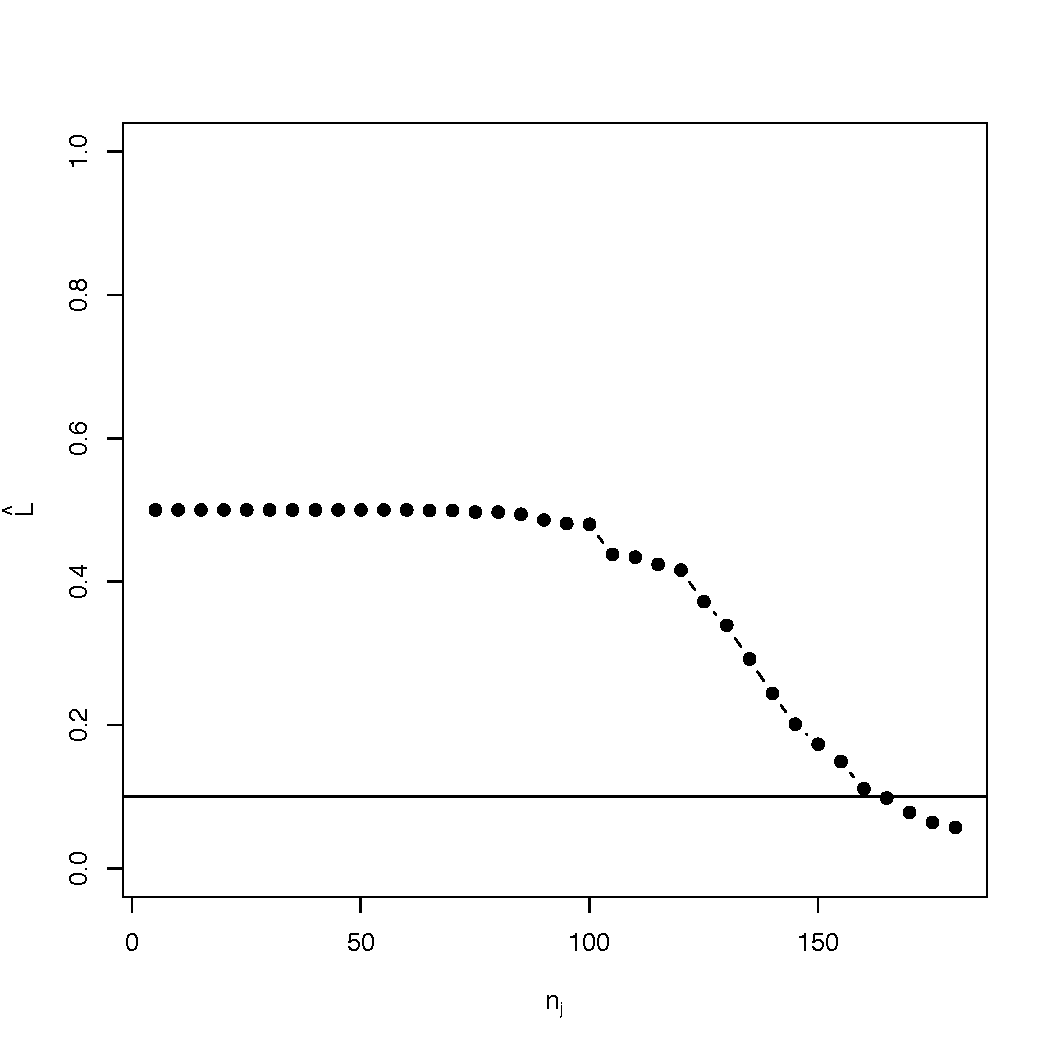
\includegraphics[width=.5\linewidth]{Lhatplot}
\caption{C.~elegans graph classification simulation results. $\hL^{1000}_{\PP}(g_n)$ is plotted as a function of class-conditional training sample size $n_j$, suggesting that for $\varepsilon=0.1$ we can determine that $\MeB$ holds with $99\%$ confidence with just a few hundred training samples generated from $\PP[M,B]$. Each dot depicts an estimate for $L_{\PP}(g_n)$; standard errors are $(L_{\PP}(g_n)(1-L_{\PP}(g_n))/1000)^{1/2}$\tr{; e}.g., $n_j = 180$ ; $k_n = 53$ ; $\hL^{1000}_{F}(g_n) = 0.057$; standard error less than 0.01. We reject $H_0: L_{\PP}(g^*) \geq 0.10$ at $\alpha=0.01$. $L_{\PP}(g^*) \approx 0$ for this simulation.
}
\label{fig1}
\end{figure}

Importantly, conducting this experiment {\it in actu} is not beyond current technological limitations. 3D superresolution imaging \cite{VaziriShank08} combined with neurite tracing algorithms \cite{HelmstaedterDenk08,Mishchenko09,LuLichtman09} allow the collection of a brain-graph within a day. Genetic manipulations, laser ablations, and training paradigms can each be used to obtain a non-wild type population for use as $M=m_1$ \cite{deBonoMaricq05}, and the class of each organism ($m_0$ vs.~$m_1$) can also be determined automatically \cite{BuckinghamSattelle08}.

\clearpage

% subsection simulation (end)



\section*{Acknowledgments}

The authors would like to acknowledge helpful discussions with J.~Lande, B.~Vogelstein, and S.~Seung. 


% \section{References}
% \bibliography{biblist}
\bibliography{/Users/jovo/Research/papers/meta/biblist}
\bibliographystyle{ieeetr}


\end{document}

